
\documentclass[12pt]{article}
% Standard ams packages
\usepackage{amsmath, amssymb, amsthm, graphicx}
\usepackage{float}
% Edit margins
\usepackage[letterpaper, margin=1in, left=0.8in]{geometry}
\usepackage{verbatim}
% Resume enumeration after a break
\usepackage{enumitem}
\makeatletter
\def\verbatim@nolig@list{\do\`\do\<\do\>\do\'\do\-}% no comma
\makeatother
%\pagenumbering{gobble}
\usepackage{tikz}
% Define macros
\global\long\def\dom{\mathop\mathrm{dom}\nolimits}   % domain
\global\long\def\Ker{\mathop\mathrm{Ker}\nolimits} % kernel
\global\long\def\Im{\mathop\mathrm{Im}\nolimits} % image
\global\long\def\C{\mathbb{C}}                       % complex
\global\long\def\R{\mathbb{R}}                       % reals
\global\long\def\Q{\mathbb{Q}}                       % rationals
\global\long\def\Z{\mathbb{Z}}                       % integers
\global\long\def\N{\mathbb{N}}                      % naturals
\global\long\def\A{\mathcal{A}}
\global\long\def\F{\mathbb{F}}
\def\div{\, \big| \,} % divides
\def\inv{^{-1}} % inverse
\def\tr{\text{Trace}} % trace
\def\GL{\text{GL}} % general linear
\def\SL{\text{SL}} % special linear
\def\char{\text{char}} % characteristic

% Generator of a group
\newcommand{\gen}[1]{\langle #1 \rangle}
\renewcommand{\qedsymbol}{\(\blacksquare\)}

\theoremstyle{plain}
\newtheorem{corollary}{Corollary}
\newtheorem{lemma}{Lemma}
\newtheorem{example}{Example}
\newtheorem{observation}{Observation}
\newtheorem{proposition}{Proposition}
\newtheorem{theorem}{Theorem}
\newtheorem{axiom}{Axiom}
\newtheorem{question}{Question}

\theoremstyle{definition}
\newtheorem{definition}{Definition}

\theoremstyle{remark}
\newtheorem{remark}{Remark}

% Quick permutation group notation (3 elements)
\newenvironment{permutation3}
{
\left(\begin{tabular}{ccc}
}
{
\end{tabular}\right)
}

% Quick permutation group notation (4 elements)
\newenvironment{permutation4}
{
\left(\begin{tabular}{cccc}
}
{
\end{tabular}\right)
}

\newcommand{\ext}[1]{% a one shot command for this display
  \hphantom{\scriptstyle#1}\bigg|{\scriptstyle#1}%
  }
% Quick permutation group notation (5 elements)
\newenvironment{permutation5}
{
\left(\begin{tabular}{ccccc}
}
{
\end{tabular}\right)
}

% Quick permutation group notation (6 elements)
\newenvironment{permutation6}
{
\left(\begin{tabular}{cccccc}
}
{
\end{tabular}\right)
}

% Quick permutation group notation (7 elements)
\newenvironment{permutation7}
{
\left(\begin{tabular}{ccccccc}
}
{
\end{tabular}\right)
}

\title{Advanced Topics: Security of HE}
\author{Bahattin Yildiz }
\begin{document}
\date{}

\maketitle
In this chapter, we will be talking about some of the advanced topics that appear heavily in implementations of Homomorphic Encryption. More precisely, we will be talking about ``lattices", ``shortest vector problem", ``LWE" and ``RLWE" cryptosystems, which form the basis of HE. These mostly determine the security of the HE implementations. We assume that the reader has already familiarized themselves with the previous material on Number Theory, Groups, Rings/Fields and Galois Theory/Cyclotomics as we will be building up on the material mentioned here.


 \section{Lattices}
\begin{definition}
A {\it lattice} is a discrete subgroup of $\mathbb{R}^n$. More precisely, a lattice is a subset $\Lambda$ of $\mathbb{R}^n$ that possesses the following two properties:
\par {\bf a)} For $\mathbf{x}, \mathbf{y} \in \Lambda$, we have $\mathbf{x}-\mathbf{y}\in \Lambda$
\par {\bf b)} There is an $\epsilon >0$ such that for all $\mathbf{x},\mathbf{y} \in \Lambda$ with $\mathbf{x}\neq \mathbf{y}$, we have $||\mathbf{x}-\mathbf{y}||>\epsilon$.
\end{definition}
\begin{remark}
Note that the second property ensures that a lattice is a ``discrete structure".
\end{remark}

\begin{example}\begin{enumerate}
    \item A classical example of a lattice is $\mathbb{Z}^n$, i.e., the set of vectors $(a_1, a_2, \dots, a_n)$ such that $a_i\in \mathbb{Z}$ for $i=1,2, \dots, n$.
    \item In particular the set $\Z$ of integers is also a lattice.

        \bigskip

    \begin{tikzpicture}
\tikzstyle{point1}=[ball color=red, circle, draw=black, inner sep=0.1cm]
\tikzstyle{point2}=[ball color=green, circle, draw=black, inner sep=0.1cm]

\node (v1) at (-6,0) [point2] {};
\node (v2) at (-5,0) [point2] {};
\node (v3) at (-4,0) [point2] {};
\node (v4) at (-3,0) [point2] {};
\node (v5) at (-2,0) [point2] [label=below:$-3$]{};
\node (v6) at (-1,0) [point2] [label=below:$-2$]{};
\node (v7) at (0,0) [point2] [label=below:$-1$]{};
\node (v8) at (1,0) [point2] [label=below:$0$]{};
\node (v9) at (2,0) [point2] [label=below:$1$]{};
\node (v10) at (3,0) [point2] [label=below:$2$]{};
\node (v11) at (4,0) [point2] [label=below:$3$]{};
\node (v12) at (5,0) [point2] {};
\node (v13) at (6,0) [point2] {};
\node (v14) at (7,0) [point2] {};
\node (v15) at (8,0) [point2] {};


\draw (v1) -- (v2) -- (v3)--(v4)--(v5)--(v6)--(v7)--(v8)--(v9)--(v10)--(v11)--(v12)--(v13)--(v14)--(v15);
\end{tikzpicture}

\bigskip


    \item Consider the set
    $$\frac{1}{2}\Z = \left \{\frac{m}{2}|m\in \Z\right \}.$$
    This contains all ``integers" as well as ``half-integers". So, even though it is defined as $\frac{1}{2}\Z$, it contains ``twice" as much as the integers. It is in fact a lattice in $\R$.

    \bigskip

    \begin{tikzpicture}
\tikzstyle{point1}=[ball color=red, circle, draw=black, inner sep=0.1cm]
\tikzstyle{point2}=[ball color=green, circle, draw=black, inner sep=0.1cm]

\node (v1) at (-6,0) [point1] {};
\node (v2) at (-5,0) [point2] {};
\node (v3) at (-4,0) [point1] [label=below:$\frac{-5}{2}$]{};
\node (v4) at (-3,0) [point2] [label=below:$-2$]{};
\node (v5) at (-2,0) [point1] [label=below:$\frac{-3}{2}$]{};
\node (v6) at (-1,0) [point2] [label=below:$-1$]{};
\node (v7) at (0,0) [point1] [label=below:$\frac{-1}{2}$]{};
\node (v8) at (1,0) [point2] [label=below:$0$]{};
\node (v9) at (2,0) [point1] [label=below:$\frac{1}{2}$]{};
\node (v10) at (3,0) [point2] [label=below:$1$]{};
\node (v11) at (4,0) [point1] [label=below:$\frac{3}{2}$]{};
\node (v12) at (5,0) [point2] [label=below:$2$]{};
\node (v13) at (6,0) [point1] [label=below:$\frac{5}{2}$]{};
\node (v14) at (7,0) [point2] {};
\node (v15) at (8,0) [point1] {};


\draw (v1) -- (v2) -- (v3)--(v4)--(v5)--(v6)--(v7)--(v8)--(v9)--(v10)--(v11)--(v12)--(v13)--(v14)--(v15);
\end{tikzpicture}

\bigskip

\item The following describes a lattice in $\R^2$:

\bigskip
\noindent
\begin{center}
    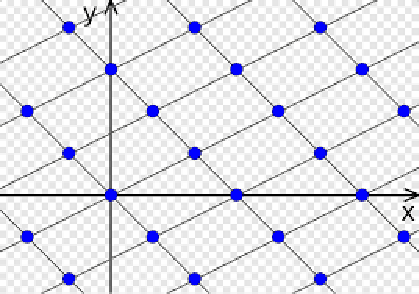
\includegraphics[scale=1.00]{images/png2pdf.pdf}
\end{center}

\end{enumerate}

\end{example}

\bigskip
\noindent
Lattices can also be defined via bases as follows.
\vspace{-0.1cm}
\begin{definition}
Let $\mathfrak{B}=\{\mathbf{b}_1, \mathbf{b}_2, \dots, \mathbf{b}_m\}$ be a set of $m$ linearly independent vectors in $\mathbb{R}^n$. Then the lattice generated by $\mathfrak{B}$ is defined as $\displaystyle{\Lambda(\mathfrak{B}) = \{x_1\mathbf{b}_1+x_2\mathbf{b}_2+\dots + x_m\mathbf{b}_m | x_i \in \mathbb{Z}\}.}$
\end{definition}

\begin{example}
\begin{enumerate}
    \item In the case when the lattice is $\Z$, a basis is given by $\{1\}$. Note that $\{-1\}$ can also be taken as a basis.
    \item In the case of $\frac{1}{2}\Z$, what can we take as a basis? Clearly both $\{\frac{1}{2}\}$ and $\{\frac{-1}{2}\}$ can taken as bases. However in this case $\{1\}$ is not a basis anymore.
    \item The following lattice has two different bases, with one being $\{u_1, u_2\}$ while the other is given by $\{v_1, v_2\}$.

    \bigskip

    \begin{center}
    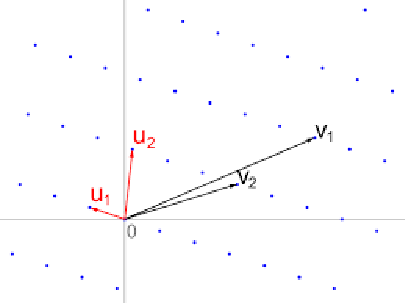
\includegraphics[scale=1.00]{images/LatticeWithBasis.pdf}
\end{center}

\bigskip
\noindent
Note that $\{u_1, v_1\}$ is not a basis, because when we draw the parallelogram formed by $u_1, v_1$, we have points that remain ``inside"
the parallelogram, which means this inside points cannot be obtained from integer linear combinations of $u_1$ and $v_1$.
\end{enumerate}
\end{example}

\bigskip
\noindent
Alternatively, a lattice  can also be defined by a matrix. If $B$ is an $m\times n$ matrix over $\mathbb{R}$ whose rows are  the basis vectors $b_i$, then
$\Lambda(\mathfrak{B}) = \Lambda(B)  = \{\mathbf{x}B|\mathbf{x}\in \mathbb{Z}^n\}.$ Note that, as will be seen later in the cryptographic applications, $\mathbb{Z}$ will be replaced by $\mathbb{Z}_q$ in some description of lattices.

\subsection{SVP: A ``hard" problem in Lattices}
Hard problems are very important in building cryptographic schemes. They can sometimes lead to ``OWF" (one-way function) which is extremely useful in securing a scheme.

Consider for example the ``integer factorization" problem. Given primes $p$ and $q$, we can easily compute $pq$, but given $n=pq$, we cannot easily find $p$ and $q$. This was the main hard problem that was used in securing the RSA cryptosystem.

Another example of a hard problem is the ``discrete logarithm" problem. Assuming that $G$ is a cyclic group with a generator $g$, given an integer $n$, we can compute $g^n$ easily. However given an element in the group that is of course of the form $g^k$ for some $k\in \Z$, finding $k$ is extremely hard. This is the basis of Diffie-Helman Key exchange.

The common theme of both these examples of hard problems is that they are deemed ``vulnerable" against quantum computing.

The main ``hard" problem in lattices is the so-called ``shortest vector problem" (SVP). There are many versions of the problem, but in essence it is the problem of finding the shortest (according to some predefined norm, usually the Euclidean norm) non-zero vector that is in a given lattice $\Lambda$.
\begin{example}
\begin{enumerate}
    \item Let us look at a very simple example. Consider the lattice $\Lambda \subseteq \Z$ that is generated by $6$ and $8$. What is the shortest vector in $\Lambda$? As you may have guessed, this problem was solved a long time ago by someone called ``Euclid". Of course, in this case the shortest vector is given by $2$ (or $-2$), which is the GCD of $6$ and $8$.
  \item If $\Lambda=\Z$, then $1$ $($or $-1$ $)$ is the shortest vector
  \item If $\Lambda = \frac{1}{2}\Z$, then $\frac{1}{2}$ $($or $\frac{-1}{2}$ $)$ is the shortest vector.
\item If $\Lambda$ is generated by the basis $\{(1,0), (0,1)\}$, then clearly $\Lambda = \Z\times \Z=\Z^2$. In this case any vector of the form
$(\pm 1,0)$ and $(0,\pm 1)$ are the shortest vectors, since $\sqrt{a^2+b^2}\geq 1$ for all $a, b\in \Z$ that are not both $0$.
\end{enumerate}
\end{example}
In general the SVP is a very hard problem and is used in the security of LWE and RLWE, on which the HE is built.

\section{LWE and RLWE}
Both the LWE and RLWE are schemes which determine the security of the FHE. We will give a broad introduction to both in this section.
\subsection{LWE}
LWE stands for ``Learning with Errors" and was first introduced by Regev in $2006$ in \cite{LWE}.

The LWE problem asks to recover a secret $\mathbf{s} \in \Z_q^n$ given a sequence of ``approximate"
random linear equations on $\mathbf{s}$. For instance, the input might be
\begin{align*}
3s_1 + 3s_2 + s_3 & \approx 10 \pmod{11}\\
s_1 + s_2 + 5s_3  & \approx 5 \pmod{11}\\
2s_1 + 2s_2 + 3s_3 & \approx 2 \pmod{11} \\
7s_1 + 8s_2 + s_3 & \approx 7 \pmod{11} \\
\vdots \\
s_1 + 2s_2 + 3s_3 & \approx 2 \pmod{11},
\end{align*}
where each equation is correct upto an additive error ($\pm 1$). The goal is to recover $\mathbf{s}$ (In this case, the answer is given by $\mathbf{s}=(1,1,3)$).

If there were no errors, we could find the answer quickly, using Gaussian Elimination. The introduction of errors into the problem makes the problem significantly more difficult.

\bigskip
\noindent
{\bf More Precise Description of the Problem:}
\\
Let $n\geq 1$ be a size parameter, $q\geq 2$ be a modulus and $\mathcal{\chi}$ be a probability distribution defined on $\Z_q$. Let $A_{\mathbf{s},\mathcal{\chi}}$ on $\Z_q^n\times  \Z_q$ be the probability distribution
obtained by choosing a vector $\mathbf{a} \in \Z_q^n$
uniformly at random, choosing $e \in \Z_q$ according to $\mathcal{\chi}$, and outputting $(\mathbf{a},\langle \mathbf{a},\mathbf{s}\rangle + e)$, where additions are performed in $\Z_q$. We say that
an algorithm solves LWE with modulus $q$ and error distribution $\mathcal{\chi}$ if, for any $\mathbf{s} \in \Z_q^n$, given an
arbitrary number of independent samples from $A_{\mathbf{s},\mathcal{\chi}}$, it outputs $\mathbf{s}$ (with high probability).

For example, in the above problem we had $\mathbf{s}=(1, 1, 3)$, $q=11$, and $\mathbf{a}_1 = (3,3,1)$, $\mathbf{a}_2 = (1,1,5)$, $\mathbf{a}_3 = (2,2,3)$, $\mathbf{a}_4 = (7,8,1)$, etc. while $e_1=1$, $e_2=-1$, $e_3=0$, $e_4=0$, etc.

There are two main variants of the problem:
\begin{enumerate}
    \item {\bf Decision LWE:} Given access to polynomially many samples of the form $(\mathbf{a}, \langle \mathbf{a}, \mathbf{s}\rangle+e)$, the decision LWE is the problem is to distinguish between these and random vectors taken from $\Z_q^{n+1}$
    \item {\bf Search LWE:} Given access to polynomially many samples of the form $(\mathbf{a}, \langle \mathbf{a}, \mathbf{s}\rangle+e)$, the search LWE is the problem of finding $\mathbf{s}$.
    \end{enumerate}

\subsection{RLWE} The RLWE problem is analogous to the LWE problem. It was proposed by
Lyubashevsky et al. in \cite{RLWE-1}. It is an algebraic variant of the learning with errors problem. The ring variant is more time- and memory-efficient to compute, so building
cryptographic primitives on top of it can lead to more efficient protocols. Just like the LWE problem, there are two versions of the RLWE problem, namely the decisional and the
search version. Both are based on the RLWE distribution for an integer $q > 2$ and
a secret s sampled from $\mathcal{\chi}$. The authors of the problem give a quantum reduction
from the approximate shortest vector problem on ideal lattices to both versions of
the RLWE problem. Informally, this means that both the decisional and search
version are hard, assuming that worst-case problems on ideal lattices are hard for
quantum computers. This hardness result makes the RLWE problem attractive in the field of cryptography.

The finalist in NIST's PQC competition is a cryptosystem based on the RLWE.

The main difference between LWE and RLWE is that in RLWE the polynomial ring is used. The underlying ring $R$ in RLWE is the quotient ring of polynomials $\Z[x]/(f(x))$, where $f(x)$ is an irreducible polynomial in $\Z[x]$ (It does not have to be monic, but in practice it is almost always taken to be monic). The actual ring over which all the operations in RLWE are done is $R_q = R/qR$, which can also be described as $\Z_q[x]/(f(x))$.

Because of many of their nice properties, cyclotomic polynomials are used in place of $f(x)$. In particular, in the original applications, the cyclotomic is chosen to be of power $2$ in which case $f(x)=x^n+1$, where $n$ is a power of $2$.

\begin{definition}(RLWE distribution). Fix a secret $\mathbf{s}\in R_q$. The RLWE distribution $A_{s,\mathcal{\chi}}$ is defined by first sampling $\mathbf{a}$ uniformly from $\R_q$, and error $e$ from $\mathcal{\chi}$ and then returning
$(\mathbf{a}, \mathbf{a}\cdot \mathbf{s} + e])$.
\end{definition}

Just like the LWE case, the two main variants of the RLWE problem are given as follows:
\begin{enumerate}
    \item {\bf Decision RLWE:} Given access to polynomially many samples uniformly chosen from $R_q^2$, the decision RLWE is the problem is to distinguish between these and $A_{s,\mathcal{\chi}}$.
    \item {\bf Search RLWE:} Given access to polynomially many samples of the form $A_{s,\mathcal{\chi}}$, the search RLWE is the problem of finding $\mathbf{s}$.
    \end{enumerate}

\section{Encryption and Decryption in HE}
\section{Addition and Multiplication in HE}
\section{Bootstrapping}
We take most of the material in this section from \cite{bootstrap}. Bootstrapping is the standard method to turn a somewhat homomorphic scheme into a fully homomorphic scheme. We are going to explain one such case for some special parameters but the general case works in the same way for other cases as well.
\subsection{The Ambient Spaces}
The scheme is defined over a ring $R = \Z[X]/F(X)$ for a monic, irreducible polynomial $F(X)$ over the integers Z (In most implementations $F(x)$ is taken to be a cyclotomic to ensure these properties). For an arbitrary integer modulus $n$ (not necessarily prime) we denote the ring
$$R_n:= R/nR = (\Z/n\Z)[X]/(F(X)) = \Z_n[x]/(F(x)).$$ one of the parameters of the scheme is the number of levels that it can handle, which we denote by $L$, and by a set of decreasing odd moduli
$$q_0\gg q_1\gg \dots \gg q_L.$$

For this particular case, we use $2$ as the plaintext modulus, meaning that the plaintext space is given by
$$R_2 = \Z_2[x]/(F(x)).$$

The ciphertext space for the $i$th level is given by $R_{q_i}^2$. The secret key is given by the pair $\mathbf{s} = (1, \mathfrak{s})$, where $\mathfrak{s}$ is a ``small" polynomial in $R$.

A level $i$ ciphertext $\mathbf{c} = (c_0, c_1)$ encrypts a plaintext polynomial $m \in R_2$ with respect to $\mathbf{s} = (1, \mathfrak{s})$ if we have the equality over $R$,
$$[\mathbf{c}, \mathbf{s}]_{q_i} = [c_0 + \mathfrak{s}c_1]_{q_i} \equiv m \pmod{2},$$
and moreover the polynomial $[c_0 + \mathfrak{s}c_1]_{q_i}$ is ``small”, i.e. all its coefficients are considerably smaller than $q_i$.

The noise-control technique in BGV uses the fact that level-$i$ ciphertext can be publicly converted into a level-$(i + 1)$ ciphertext (with respect to the same secret key), and that this transformation reduces the noise in the ciphertext roughly by a factor of $q_{i+1}/q_i$.

Secret keys are also associated with levels, and the public key includes some additional information that (roughly speaking) makes it possible to convert a ciphertext with respect to level-$i$ key $\mathbf{s}_i$ into a ciphertext with respect to level-$(i + 1)$ key $s_{i+1}$.

For the bootstrapping purposes, we will only be interested in the secret keys at level $L$ and level $zero$;
which we will denote by $\mathbf{s}$ and $\tilde{\mathbf{s}}$ respectively.

\subsection{General Picture of Bootstrapping}
For bootstrapping, we have as input a level-$L$ ciphertext (i.e. a vector $\mathbf{c} \in R_{q_L}$ modulo the smallest modulus $q_L$). This means that the noise-control technique can no longer be applied to reduce the noise, hence (essentially) no more homomorphic operations can be performed on this ciphertext. To enable further computation, we must therefore ``recrypt” the ciphertext $\mathbf{c}$, to obtain a new ciphertext that encrypts the same element of $R$ with respect to some lower level $i <L$.

{\bf An Observation:} The decryption at level $L$ can be made more efficient when
$q_L = 2^r+1$ for an integer $r$, and moreover
the coefficients of $Z = \langle \mathbf{c}, \mathbf{s}\rangle \pmod{F(X)}$ are much smaller than $q_L^2$ in magnitude.
In particular if $z$ is one of the coefficients of the polynomial $Z$ then $[[z]_{q_L}]_2$ can be
computed as $z\langle r \rangle\oplus z\langle 0 \rangle$, where $z\langle i\rangle$ is the $i$th bit of $z$.

The more precise picture is given by the following lemma and its corollary:
\begin{lemma}
Let $q = 2^r + 1$ for a positive integer $r$, and let $z$ be a non-negative integer
smaller than $\frac{q^2}{2}-q$, such that $[z]_q$ is also non-negative, i.e., $[z]q \in [0, \frac{q}{2}]$.  Then $[[z]_q]_2=z\langle r \rangle\oplus z\langle 0 \rangle$. \end{lemma}
The corollary extends this a little further:
\begin{corollary}
Let $r\geq 3$ and $q = 2^r+1$ and let $z$ be an integer with absolute value
smaller than $\frac{q^2}{4}-q$, such that $[z]_q \in (\frac{-q}{4}, \frac{q}{4})$. Then $[[z]_q]_2=z\langle r \rangle\oplus z\langle r-1 \rangle \oplus z\langle 0 \rangle$.
\end{corollary}

{ \bf Working Modulo $2^r+1$:} Since we are only interested in the contents of bit positions $0$, $r-1$, and $r$ in the polynomial $Z$, we can compute $Z$ modulo $2^r+1$ rather than over the integers. Our simplified decryption of a ciphertext vector $\mathbf{c} = (c_0, c_1)$ proceeds as
follows:
\begin{enumerate}
    \item Compute $Z \leftarrow [\langle\mathbf{c}, \mathbf{s}\rangle \pmod{F(x)}]_{2^r+1}$;
    \item Recover the $0-1$ plaintext polynomial $a =[z\langle r \rangle\oplus z\langle r-1 \rangle \oplus z\langle 0 \rangle]_2$.
\end{enumerate}

\subsection{Encrypting the secret Key}
 Encrypting the secret key is the main step in bootstrapping. Bootstrapping only comes into the picture once we reach the smallest modulus $q_L$ so that we can no longer reduce the noise by modulus-switching.

 In recent works, improvements have been made for the bootstrapping. However, the main idea remains the same. We will give a special such case here.

Denoting by $\tilde{\mathbf{s}}$ the level-$0$ secret-key and by $q_0$ the largest
modulus, a ciphertext encrypting $a \in \Z_{2^r+1}[X]/F(X)$ with respect to $\tilde{\mathbf{s}}$ and $q_0$ is a $2$-vector $\tilde{c}$ over $\Z_{q_0}[X]/F(X)$ such that $|[\langle \tilde{\mathbf{c}},\tilde{\mathbf{s}}\rangle \pmod{F(X)}]_{q_0}| \ll q_0$ and  $|[\langle \tilde{\mathbf{c}},\tilde{\mathbf{s}}\rangle \pmod{F(X)}]_{q_0}| \equiv a \pmod{2^{r+1}}$.

We recall that the ciphertext before bootstrapping is with respect to secret key $\mathbf{s}$ and modulus $q_L = 2^r + 1$. Denoting $\mathbf{s} = (1, \mathfrak{s})$ and $\mathfrak{s}(X) =\sum_{j=0}^{d-1}\mathfrak{s}_jX^j$, we encode for each $j$ the coefficient $\mathfrak{s}_j$ as the constant polynomial $\mathfrak{s}_j \in \Z_{2^{r+1}}[X]/(F(X))$ (i.e., the degree-$d$ polynomial whose free term is $\mathfrak{s}_j \in [-2^r + 1, 2^r]$ and all the other coefficients are zero.) Then for each $j$ we include in the public key a ciphertext $\tilde{\mathbf{c}}_j$ that encrypts this constant polynomial $\mathfrak{s}_j$ with respect to $\tilde{\mathbf{s}}$ and $q_0$.

{\bf Computing $Z$ Homomorphically:} Given the $q_L$-ciphertext $\mathbf{c} = (c_0, c_1)$ (that encrypts a plaintext polynomial $a \in  \F_2[X]/(F(X))$, we use the encryption of $\mathbf{s}$ from the public key to compute the simple decryption formula from above. Namely, we compute an encryption of
$Z = [\langle\mathbf{c}, \mathbf{s}\rangle \pmod{F(X)}]_{2^r+1}$.

\subsection{Extracting Top and Bottom Bits}
\begin{thebibliography}{99}

 \bibitem{bootstrap} C. Gentry, S. Halevi and N. Smart, ``Better Bootstrapping in Fully Homomorphic Encryption".
\bibitem{RLWE-1} V. Lyubashevsky, C. Peikert, and O. Regev, ``On ideal lattices and learning with errors over rings", In Annual International Conference on the Theory and Applications of Cryptographic Techniques, pages 1–23. Springer, 2010

\bibitem{RLWE} V. Lyubashevsky, C. Peikert, and O. Regev, ``A toolkit for ring-lwe cryptography", In Annual International Conference on the Theory and Applications of Cryptographic Techniques, pages 35–54. Springer, 2013.

\bibitem{LWE} O. Regev, ``Lattice-based cryptography". In CRYPTO, pages 131–141. 2006.
% \bibitem{GHS} C. Gentry, S. Halevi and N. Smart, ``Fully Homomorphic
% Encryption with Polylog Overhead"

% \bibitem{Des} S. Halevi and V. Shoup, ``HELib Design Principles"
\end{thebibliography}

\end{document}
